\chapter{EXPERIMENT RESULT WITH PROTOTYPE}

%\section{Introduction to Corn Experiment Field in Hebi}

%介绍鹤壁试验田的具体信息
%试验田相对于正常生产经营的农场特别小,大概只有足球场大,大型农机不适用
%试验田现在的自动化程度还不及平均水平,因为要求精确度很高,所以很多作业都要靠人工
%相对于引进大型农机,在现有的农机上进行低成本改造更可行
%围绕试验田相关需求设计实验

\section{Image Processing}
%在不同的光强,距离测试
%在光度学中是没有“光强”这样一个概念的。常用的光学量概念有发光强度、光照度、光出射度和光亮度。“光强”只是一个通俗的说法很难说对应哪一个光度学概念。以上所说的几个概念都是有严格的物理定义的:发光强度:光源在单位立体角内发出的光通量单位是坎德拉即每球面度1流明。光照度:被照明面单位面积上得到的光通量单位是勒克斯即每平方米1流明。光出射度:光源单位面积上发出的光通量单位与光照度相同。光亮度:单位面积上沿法线方向的发光强度或称单位面积在其法线方向上单位立体角内发出的光通量单位是尼特即每平方米每球面度1流明。由于发光强度、光亮度与方向有关容易推导出:各个方向上光亮度相同的光源其发光强度是方向的余弦函数在法线方向上发光强度最大称为余弦辐射体也叫朗伯光源。各个方向上发光强度都相等的光源其光亮度就是不等的。
The image processing algorithm is the core of this guidance system. Both day time, high-intensity surrounding light, and night time, low-intensity surrounding light were tested different distances. The surrounding light was measured in the unit of illuminance, $LUX$, and the distance was measured in meters.% In addition, rain is considered as a possible condition for the farming season. Therefore, an experiment was conducted in the rain with the rainfall rate measured in $mm/hours$. Snowy weather is not considered.

The goal of testing the image processing algorithm is to find out the error between the real position and the estimated position of the laser spot. The real positions are measured from the original photo, while the estimated position is the result generated by the algorithm. For each distance, five different locations on the curtain were tested. The error is calculated by averaging the magnitude of the distance between the real and estimated points. 

\begin{table}[ht!]
\begin{center}
\caption{The Average Error at day ($760,000LUX$)}
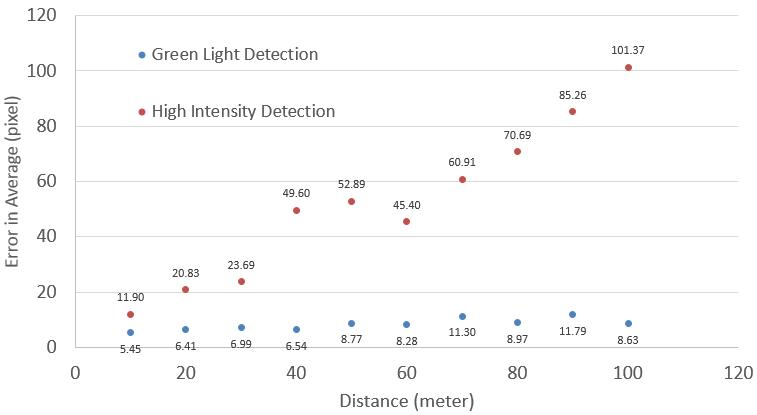
\includegraphics[scale = 0.6]{pics/dataday.jpg}
\end{center}
\end{table}

Direct sun light is too strong compared to the laser pointer, so it must be prevented. The illuminance of surrounding light in shadow is about $760,000LUX$, which is good enough for the green light detection to work. Table 6.1 shows the experiment results under daylight shadows. The high light intensity detection was defective beyond $30m$ while the green light detection worked properly all the time.  


\begin{table}[ht!]
\begin{center}
\caption{The Average Error at Night ($20LUX$)}
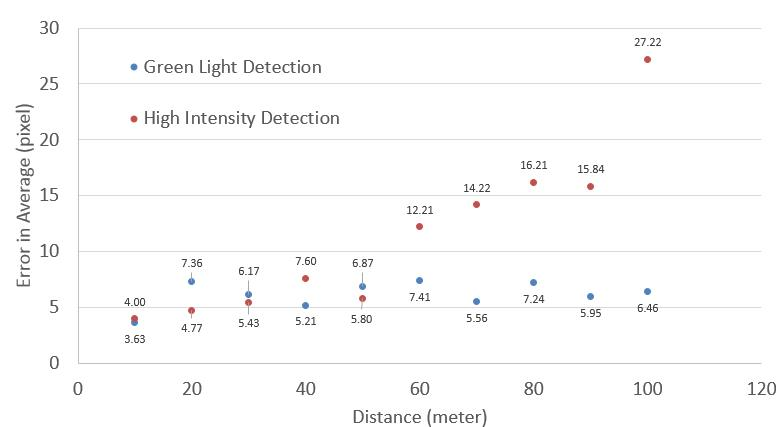
\includegraphics[scale = 0.6]{pics/datanight.jpg}
\end{center}
\end{table}

Table 6.2 shows the results at night for the same procedure of the experiment. The illuminace of surrounding light is only $20LUX$. Green light detection still worked all the time, but the high light intensity was slightly off beyond $50m$.

In both experiments, the green light detection was slightly unstable, especially during the night, because of the laser pointer. This common $5mW$ laser pointer scatters seriously as the range goes far. This starts to affect the detection from $70m$ and farther in the day, and detection is even more affected at night because under a weak surrounding light, any green light noise on the curtain will be detected. Therefore, a more precise laser pointer with less scattering at greater distances is necessary for the real device.
%激光在远距离散射严重

\section{Stepper Motor Control}

%\subsection{Motor Speed vs. Control Signal Frequency}

%\subsection{Motor speed vs. Input Current}

\subsection{Motor Speed}

The motor speed was measured with motor control code only, so that the image processing part will not slow the motor down. The motion of the motor was controlled directly by user input, and it ran at full speed. The time was counted in the program and the displacement was measured by a ruler. The loop ran for 500 cycles, and the time consumed was $3182114\mu s$, or about $3.13s$. The displacement measured was about $20cm$. The result is $6.39cm/s$.  

\subsection{Loop Speed}

Usually loop speed is insignificant, but it is considerable for a 900MHz CUP. The loop speed was measured in the program, so it is considered accurate. The motor control loop has a good run speed, which is $6260\mu s/loop$, but the image processing loop is much slower. Its loop speed is $170608\mu s/loop$, which means it takes about $0.17s$ for each loop. If both the image processing and motor control code run together, it will take $176868\mu s$ for each loop. It would need $44.217s$ to make a $10cm$ movement, which is unacceptable. Therefore, multi-thread programming is necessary. If the image processing and motor control parts run in two threads, the motor is able to run at full speed while the image processing part sends a command every $0.17s$. It would only need $1.56s$ to make a $10cm$ movement, which is much better.

%\subsection{Multi-thread Programming}

\subsection{Reaction Time}

The typical operating speed of a farm tractor is between 5 and 10$km/h$, which is about $1.39-2.78m/s$. The laser guidance system has to find and correct the error in a limited time. Since the loop speed for image processing is $0.17s/loop$, the queuing time for an incoming frame is from $0s$ to $0.17s$, and the analyzing time is $0.17s$. Hence the reaction time is $0.17-0.34s + 0.16cm/s$. For example, the time needed to correct a $5cm$ is $0.97-1.14s$. However, the tractor can move over $1m$ in this time window. Therefore, hardware more powerful than this prototype will be needed in the real device.


%\subsection{Vehicle Moving Speed Estimation}

%\section{Practical Application Parameters Prediction}
%预测实际情况中所需电子元件的参数
%通过 农机工作时的移动速度 和 实际需要的reaction time 
%推算出 马达扭矩,速度 以及 microprocessor的处理速度
%再通过 马达和microprocessor的功率 推算出所需电源
%预测 sliding track需要的长度
%预测 投影布的大小